\documentclass[12pt]{article}


\usepackage[T1]{fontenc}
\usepackage[polish]{babel}
\usepackage[utf8]{inputenc}
\usepackage{lmodern}
\selectlanguage{polish}
\usepackage{graphicx}

\title{Styczna do wykresu funkcji}
\date{}
\begin{document}
\maketitle
\noindent
Niech funkcja \textit{f} będzie określona w otoczeniu \textit{U}($x_{0}$) oraz niech będzie różniczkowalna w samym punkcie $x_0$. Ponadto niech \textit{h} będzie liczbą rzeczywistą, dla której ($x_0$+\textit{h}) $\in$ \textit{U}($x_{0}$). Rozważmy \textit{P}$\left(x_0, f(x_0)\right)$ oraz \textit{Q}$\left(x_0+h, f(x_0+h)\right)$ należące do wykresu funkcji \textit{f}. Przez te punkty prowadzimy prostą (rysunek poniżej przedstawia przypadek \textit{h}>0).
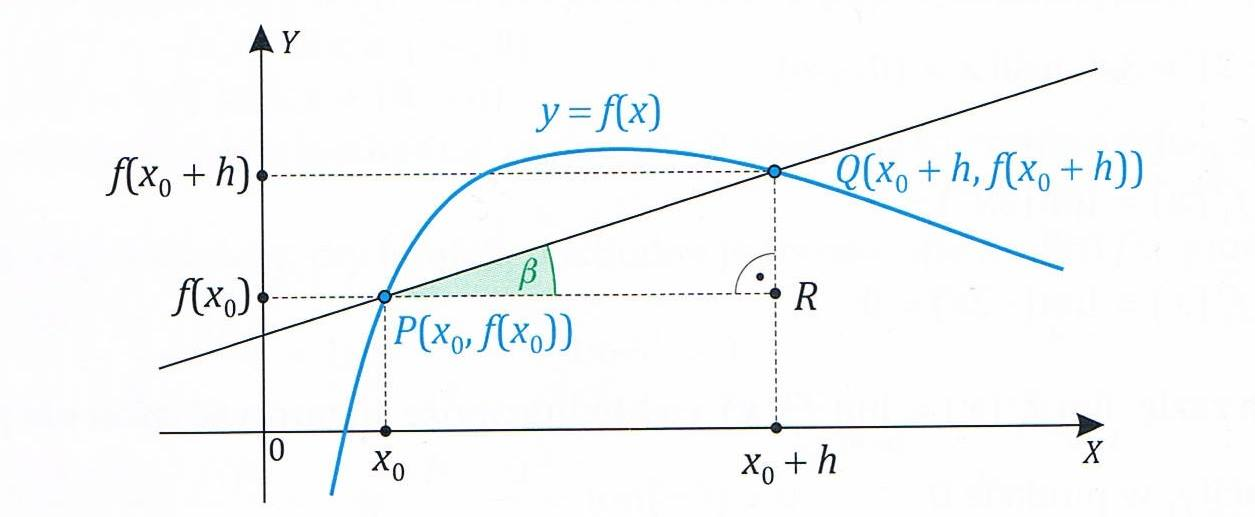
\includegraphics[height=3cm]{zdj1.jpg}
\end{document}